\documentclass[twoside]{book}

% Packages required by doxygen
\usepackage{fixltx2e}
\usepackage{calc}
\usepackage{doxygen}
\usepackage[export]{adjustbox} % also loads graphicx
\usepackage{graphicx}
\usepackage[utf8]{inputenc}
\usepackage{makeidx}
\usepackage{multicol}
\usepackage{multirow}
\PassOptionsToPackage{warn}{textcomp}
\usepackage{textcomp}
\usepackage[nointegrals]{wasysym}
\usepackage[table]{xcolor}

% Font selection
\usepackage[T1]{fontenc}
\usepackage[scaled=.90]{helvet}
\usepackage{courier}
\usepackage{amssymb}
\usepackage{sectsty}
\renewcommand{\familydefault}{\sfdefault}
\allsectionsfont{%
  \fontseries{bc}\selectfont%
  \color{darkgray}%
}
\renewcommand{\DoxyLabelFont}{%
  \fontseries{bc}\selectfont%
  \color{darkgray}%
}
\newcommand{\+}{\discretionary{\mbox{\scriptsize$\hookleftarrow$}}{}{}}

% Page & text layout
\usepackage{geometry}
\geometry{%
  a4paper,%
  top=2.5cm,%
  bottom=2.5cm,%
  left=2.5cm,%
  right=2.5cm%
}
\tolerance=750
\hfuzz=15pt
\hbadness=750
\setlength{\emergencystretch}{15pt}
\setlength{\parindent}{0cm}
\setlength{\parskip}{3ex plus 2ex minus 2ex}
\makeatletter
\renewcommand{\paragraph}{%
  \@startsection{paragraph}{4}{0ex}{-1.0ex}{1.0ex}{%
    \normalfont\normalsize\bfseries\SS@parafont%
  }%
}
\renewcommand{\subparagraph}{%
  \@startsection{subparagraph}{5}{0ex}{-1.0ex}{1.0ex}{%
    \normalfont\normalsize\bfseries\SS@subparafont%
  }%
}
\makeatother

% Headers & footers
\usepackage{fancyhdr}
\pagestyle{fancyplain}
\fancyhead[LE]{\fancyplain{}{\bfseries\thepage}}
\fancyhead[CE]{\fancyplain{}{}}
\fancyhead[RE]{\fancyplain{}{\bfseries\leftmark}}
\fancyhead[LO]{\fancyplain{}{\bfseries\rightmark}}
\fancyhead[CO]{\fancyplain{}{}}
\fancyhead[RO]{\fancyplain{}{\bfseries\thepage}}
\fancyfoot[LE]{\fancyplain{}{}}
\fancyfoot[CE]{\fancyplain{}{}}
\fancyfoot[RE]{\fancyplain{}{\bfseries\scriptsize Generated by Doxygen }}
\fancyfoot[LO]{\fancyplain{}{\bfseries\scriptsize Generated by Doxygen }}
\fancyfoot[CO]{\fancyplain{}{}}
\fancyfoot[RO]{\fancyplain{}{}}
\renewcommand{\footrulewidth}{0.4pt}
\renewcommand{\chaptermark}[1]{%
  \markboth{#1}{}%
}
\renewcommand{\sectionmark}[1]{%
  \markright{\thesection\ #1}%
}

% Indices & bibliography
\usepackage{natbib}
\usepackage[titles]{tocloft}
\setcounter{tocdepth}{3}
\setcounter{secnumdepth}{5}
\makeindex

% Hyperlinks (required, but should be loaded last)
\usepackage{ifpdf}
\ifpdf
  \usepackage[pdftex,pagebackref=true]{hyperref}
\else
  \usepackage[ps2pdf,pagebackref=true]{hyperref}
\fi
\hypersetup{%
  colorlinks=true,%
  linkcolor=blue,%
  citecolor=blue,%
  unicode%
}

% Custom commands
\newcommand{\clearemptydoublepage}{%
  \newpage{\pagestyle{empty}\cleardoublepage}%
}

\usepackage{caption}
\captionsetup{labelsep=space,justification=centering,font={bf},singlelinecheck=off,skip=4pt,position=top}

%===== C O N T E N T S =====

\begin{document}

% Titlepage & ToC
\hypersetup{pageanchor=false,
             bookmarksnumbered=true,
             pdfencoding=unicode
            }
\pagenumbering{alph}
\begin{titlepage}
\vspace*{7cm}
\begin{center}%
{\Large My Project }\\
\vspace*{1cm}
{\large Generated by Doxygen 1.8.14}\\
\end{center}
\end{titlepage}
\clearemptydoublepage
\pagenumbering{roman}
\tableofcontents
\clearemptydoublepage
\pagenumbering{arabic}
\hypersetup{pageanchor=true}

%--- Begin generated contents ---
\chapter{Namespace Index}
\section{Namespace List}
Here is a list of all namespaces with brief descriptions\+:\begin{DoxyCompactList}
\item\contentsline{section}{\mbox{\hyperlink{namespaceserver}{server}} }{\pageref{namespaceserver}}{}
\item\contentsline{section}{\mbox{\hyperlink{namespaceserver_1_1_scraper}{server.\+Scraper}} }{\pageref{namespaceserver_1_1_scraper}}{}
\item\contentsline{section}{\mbox{\hyperlink{namespaceserver_1_1_scraper_1_1data}{server.\+Scraper.\+data}} }{\pageref{namespaceserver_1_1_scraper_1_1data}}{}
\item\contentsline{section}{\mbox{\hyperlink{namespaceserver_1_1_scraper_1_1scrape}{server.\+Scraper.\+scrape}} }{\pageref{namespaceserver_1_1_scraper_1_1scrape}}{}
\end{DoxyCompactList}

\chapter{Hierarchical Index}
\section{Class Hierarchy}
This inheritance list is sorted roughly, but not completely, alphabetically\+:\begin{DoxyCompactList}
\item Form\begin{DoxyCompactList}
\item \contentsline{section}{server.\+Input\+Form}{\pageref{classserver_1_1_input_form}}{}
\end{DoxyCompactList}
\end{DoxyCompactList}

\chapter{Class Index}
\section{Class List}
Here are the classes, structs, unions and interfaces with brief descriptions\+:\begin{DoxyCompactList}
\item\contentsline{section}{\mbox{\hyperlink{classserver_1_1_scraper_1_1scrape_1_1_scraper}{server.\+Scraper.\+scrape.\+Scraper}} \\*C\+L\+A\+S\+S\+ES \# }{\pageref{classserver_1_1_scraper_1_1scrape_1_1_scraper}}{}
\end{DoxyCompactList}

\chapter{File Index}
\section{File List}
Here is a list of all files with brief descriptions\+:\begin{DoxyCompactList}
\item\contentsline{section}{\mbox{\hyperlink{____init_____8py}{\+\_\+\+\_\+init\+\_\+\+\_\+.\+py}} }{\pageref{____init_____8py}}{}
\item\contentsline{section}{\mbox{\hyperlink{data_8py}{data.\+py}} }{\pageref{data_8py}}{}
\item\contentsline{section}{\mbox{\hyperlink{scrape_8py}{scrape.\+py}} \\*File that contains all scraping functionality }{\pageref{scrape_8py}}{}
\end{DoxyCompactList}

\chapter{Namespace Documentation}
\hypertarget{namespace_flask}{}\section{Flask Namespace Reference}
\label{namespace_flask}\index{Flask@{Flask}}


Documentation for the Server.  




\subsection{Detailed Description}
Documentation for the Server. 
\chapter{Class Documentation}
\hypertarget{classserver_1_1_input_form}{}\section{server.\+Input\+Form Class Reference}
\label{classserver_1_1_input_form}\index{server.\+Input\+Form@{server.\+Input\+Form}}


C\+L\+A\+S\+S\+ES.  


Inheritance diagram for server.\+Input\+Form\+:\begin{figure}[H]
\begin{center}
\leavevmode
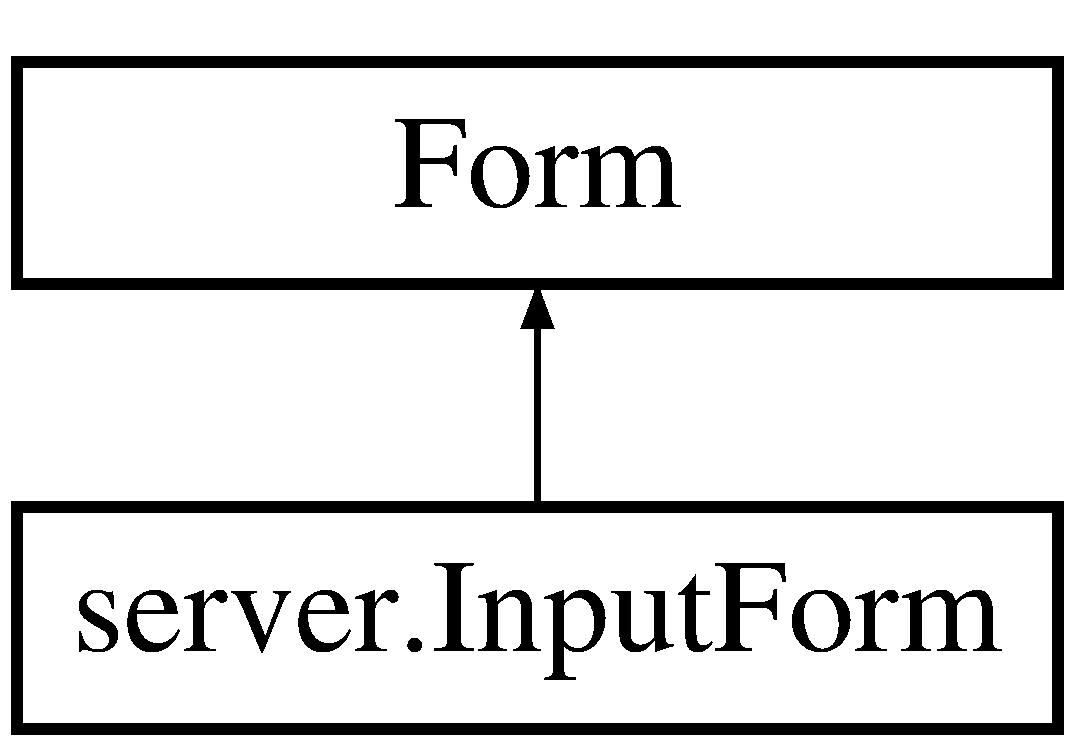
\includegraphics[height=2.000000cm]{classserver_1_1_input_form}
\end{center}
\end{figure}
\subsection*{Static Public Attributes}
\begin{DoxyCompactItemize}
\item 
\mbox{\Hypertarget{classserver_1_1_input_form_aeb69cc1418487bba68a254b916fca1f8}\label{classserver_1_1_input_form_aeb69cc1418487bba68a254b916fca1f8}} 
{\bfseries searchquery} = String\+Field(u\textquotesingle{}Enter Your Search\+:\textquotesingle{}, validators = \mbox{[}validators.\+input\+\_\+required()\mbox{]})
\end{DoxyCompactItemize}


\subsection{Detailed Description}
C\+L\+A\+S\+S\+ES. 

\mbox{\hyperlink{classserver_1_1_input_form}{Input\+Form}}

Form that Takes the String(s) Given as Input 

The documentation for this class was generated from the following file\+:\begin{DoxyCompactItemize}
\item 
\mbox{\hyperlink{server_8py}{server.\+py}}\end{DoxyCompactItemize}

\chapter{File Documentation}
\hypertarget{server_8py}{}\section{server.\+py File Reference}
\label{server_8py}\index{server.\+py@{server.\+py}}


Server run File that provides the main interface between our app and th Server Includes routing Information and Rendering of H\+T\+ML.  


\subsection*{Classes}
\begin{DoxyCompactItemize}
\item 
class \mbox{\hyperlink{classserver_1_1server_1_1_input_form}{server.\+server.\+Input\+Form}}
\begin{DoxyCompactList}\small\item\em C\+L\+A\+S\+S\+ES. \end{DoxyCompactList}\end{DoxyCompactItemize}
\subsection*{Namespaces}
\begin{DoxyCompactItemize}
\item 
 \mbox{\hyperlink{namespaceserver_1_1server}{server.\+server}}
\item 
 \mbox{\hyperlink{namespace_flask}{Flask}}
\begin{DoxyCompactList}\small\item\em Documentation for the Server \mbox{\hyperlink{namespace_flask}{Flask}} is a Microframework for Web Development thtat Utilizes Python. \end{DoxyCompactList}\end{DoxyCompactItemize}
\subsection*{Functions}
\begin{DoxyCompactItemize}
\item 
def \mbox{\hyperlink{namespaceserver_1_1server_a59e9bd350bd3f6864626e826a5d07e61}{server.\+server.\+Handle\+Data}} (data)
\begin{DoxyCompactList}\small\item\em Handle \end{DoxyCompactList}\item 
def \mbox{\hyperlink{namespaceserver_1_1server_a06b6b48a36458a5e63d37667433c2080}{server.\+server.\+Create\+Dict}} (name)
\begin{DoxyCompactList}\small\item\em Function. \end{DoxyCompactList}\item 
def \mbox{\hyperlink{namespaceserver_1_1server_ab3d96b92729f42de2866e0cb876a0a71}{server.\+server.\+index}} ()
\begin{DoxyCompactList}\small\item\em R\+O\+U\+T\+ES. \end{DoxyCompactList}\item 
def \mbox{\hyperlink{namespaceserver_1_1server_ae5d697d5408aeb2f94e2aa610a4706aa}{server.\+server.\+search}} ()
\item 
def \mbox{\hyperlink{namespaceserver_1_1server_a7bdc96668852473d18262dd1185ac3d9}{server.\+server.\+about}} ()
\begin{DoxyCompactList}\small\item\em Function \char`\"{}/about\char`\"{}. \end{DoxyCompactList}\item 
def \mbox{\hyperlink{namespaceserver_1_1server_a83a8086e94730016efda959e40b9cfaf}{server.\+server.\+results}} ()
\end{DoxyCompactItemize}
\subsection*{Variables}
\begin{DoxyCompactItemize}
\item 
\mbox{\hyperlink{namespaceserver_1_1server_abe540ab6e7c9bffd61dda91273e699e2}{server.\+server.\+app}} = Flask(\+\_\+\+\_\+name\+\_\+\+\_\+, static\+\_\+folder=\char`\"{}../static/dist\char`\"{}, template\+\_\+folder=\char`\"{}../static\char`\"{})
\item 
\mbox{\hyperlink{namespaceserver_1_1server_addf5a8b97b626d4622f3fb2b2f8065ab}{server.\+server.\+debug}}
\item 
\mbox{\hyperlink{namespaceserver_1_1server_a1e0984522028dec04483b66d00e8b6b6}{server.\+server.\+methods}}
\begin{DoxyCompactList}\small\item\em Class \char`\"{}/search\char`\"{}. \end{DoxyCompactList}\item 
\mbox{\hyperlink{namespaceserver_1_1server_a70d8440bb9056abff06b917ecacce061}{server.\+server.\+secret\+\_\+key}}
\begin{DoxyCompactList}\small\item\em Runs the Server. \end{DoxyCompactList}\end{DoxyCompactItemize}


\subsection{Detailed Description}
Server run File that provides the main interface between our app and th Server Includes routing Information and Rendering of H\+T\+ML. 

Runs the Landscrape Main Server.
%--- End generated contents ---

% Index
\backmatter
\newpage
\phantomsection
\clearemptydoublepage
\addcontentsline{toc}{chapter}{Index}
\printindex

\end{document}
